\documentclass[conference]{IEEEtran}

\usepackage[colorlinks,allcolors=blue]{hyperref}
\usepackage{amsfonts}
\usepackage{graphicx}

\begin{document}

    \title{A formal theory of digital twins}

    \author{
        \IEEEauthorblockN{Georg Hackenberg} 
        \IEEEauthorblockA{School of Engineering\\University of Applied Sciences Upper Austria\\4600 Wels, Austria} 
        \and 
        \IEEEauthorblockN{Alican Tüzün} 
        \IEEEauthorblockA{Josef Ressel Center for Data-Driven Innovation in Business Modeling\\University of Applied Sciences Upper Austria\\4xxx Steyr, Austria}
    }
   
    \maketitle

    \begin{abstract}
        TODO
    \end{abstract}

    \section{Introduction}
    \label{section:introduction}
    TODO~\cite{asf}

    \subsection{Research objective}
    More systematic development of high-quality digital twins in different application domains.

    \subsection{Research question}
    Unambiguous definition of the term "digital twin"?

    \subsection{Research methodology}
    Literature review~\ref{section:related} + formalization~\ref{section:theory} + discussion~\ref{section:discussion}.

    \section{Related work}
    \label{section:related}
    TODO

    \section{A digital twin theory}
    \label{section:theory}
    In the following, we introduce a formal theory of digital twins.
    We start with introducing core concepts in Section~\ref{section:theory-core}.
    Then, on top of the core concepts we build a theory of the real world in Section~\ref{section:theory-world}.
    Finally, on top of the theory of the real world we derive a theory of digital twins in Section~\ref{section:theory-twin}.

    \subsection{Core concepts}
    \label{section:theory-core}

    \begin{figure}[htbp]
        \centering
        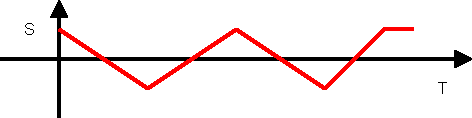
\includegraphics{./figures/theory-core.pdf}
        \caption{Illustration of core concepts}
        \label{figure:theory-core}
    \end{figure}

    The core concepts include the notion of time, the notion of state, and the notion of behavior.

    \subsubsection{Time}
    In our theory we do not prescribe a specific model of time such as discrete or continuous.
    We rather employ a generic approach, where different models of time can be plugged in easily.
    In this generic approach, time is defined as some (not further specified) set
    \[
        T.
    \]

    \subsubsection{State}
    Similar to the above case, we do not prescribe a specific model of state such as subatomic, atomic, molecular, mechanical, electrical, digital, etc.
    Again we employ a generic approach, where various models of state can be plugged in later.
    In this generic approach state is defined as some (not further specified) set
    \[
        S.
    \]

    \subsubsection{Behavior}
    Finally, we include a generic model of how state changes over time.
    Analogous to the previous two cases, concrete models of time and state can be plugged in easily.
    In our approach, a behavior is a mapping from the time domain to the state domain, i.e.
    \[
        \overrightarrow{S}: T \rightarrow S.
    \]

    \subsection{TODO}
    TODO

    \subsubsection{Observer}
    TODO

    \subsubsection{Observation}
    TODO

    \subsubsection{Event}
    TODO time point and time span (observer dependent)

    \subsection{Our model of the real world}
    \label{section:theory-world}

    \begin{figure}[htbp]
        \centering
        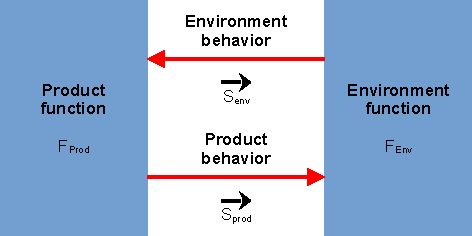
\includegraphics{./figures/theory-world.pdf}
        \caption{Illustration of real world concepts}
        \label{figure:theory-world}
    \end{figure}

    Based on the concepts of time, state, and behavior we build our model of the real world.
    This model distinguishes between a product and its environment.
    For both the product and its environment we define their states and their functions.
    Finally, we explain the concept of world behavior.

    \subsubsection{World state}
    TODO
    \[
        S_{World} = (S_{Prod}, S_{Env}).
    \]

    \subsubsection{Product state}
    In our theory, the product state describes the product perfectly at a particular point in time.
    We assume perfect knowledge in this representation and, hence, the representation is only a theoretical construct.
    Mathematically, the product state is defined as set
    \[
        S_{Prod}.
    \]

    \subsubsection{Environment state}
    Similarly, the environment state describes the environment perfectly at a particular point in time.
    Again we assume perfect knowledge in this purely theoretical representation.
    Hence, the environment state is defined mathematically as set
    \[
        S_{Env}.
    \]

    \subsubsection{World behavior}
    TODO
    \[
        \overrightarrow{S_{World}} = (\overrightarrow{S_{Prod}}, \overrightarrow{S_{Env}})
    \]

    \subsection{TODO}
    TODO

    \subsubsection{Input}
    TODO

    \subsubsection{Output}
    TODO

    \subsubsection{Function}
    TODO
    
    %\subsubsection{Product function}
    %Based on product and environment state we can define the product function.
    %The product function describes the logic of how the product reacts to the environment.
    %This logic can be described as mapping from environment behavior to product behavior, i.e.
    %\[
    %    F_{Prod}: \overrightarrow{S_{Env}} \rightarrow \overrightarrow{S_{Prod}}
    %\]

    %\subsubsection{Environment function}
    %Similarly, we can define the environment function.
    %The environment function describes the logic of how the environment reacts to the product.
    %Hence, this logic can be described as mapping from product behavior to environment behavior, i.e.
    %\[
    %    F_{Env}: \overrightarrow{S_{Prod}} \rightarrow \overrightarrow{S_{Env}}
    %\]

    %\subsubsection{World behavior}
    %Finally, based on product state and function as well as environment state and function we introduce world behavior.
    %In our theory, world behavior is a combination of consistent product and environment behavior.
    %We express world behavior as tuple
    %\[
    %    B_{World} = (\overrightarrow{S_{Prod}}, \overrightarrow{S_{Env}})
    %\]
    %such that the environment behavior $\overrightarrow{S_{Env}}$ is the result of product behavior $\overrightarrow{S_{Prod}}$, i.e.
    %\[
    %    \overrightarrow{S_{Env}} = F_{Env}(\overrightarrow{S_{Prod}})
    %\]
    %and, adversely, the product behavior $\overrightarrow{S_{Prod}}$ is the result of environment behavior $\overrightarrow{S_{Env}}$, i.e.
    %\[
    %    \overrightarrow{S_{Prod}} = F_{Prod}(\overrightarrow{S_{Env}}).
    %\]

    \subsection{Our model of digital twins}
    \label{section:theory-twin}
    TODO

    \section{Discussion}
    \label{section:discussion}
    TODO

    \section{Conclusion}
    \label{section:conclusion}
    TODO
    
    \bibliography{main}
    \bibliographystyle{plain}
    
\end{document}